\documentclass{article}
\usepackage{graphicx} % Required for inserting images
\usepackage{amsmath,amssymb,amsthm}
\usepackage{physics}
\usepackage{graphicx,float}
\graphicspath{{images/}}
\usepackage[none]{hyphenat}
\usepackage{blindtext}
\usepackage{parskip}
\usepackage[letterpaper,top=3cm, left= 3cm,bottom=3cm]{geometry}
\usepackage{subcaption}

\title{Exploring Accumulations of Changes}
\author{Polaris}
\date{2025/06/23}

\begin{document}

\maketitle

Problem: Consider this velocity-time graph, where the vertical axis is velocity in km/h, the horizontal axis is time in hours, find the distance the car travels

\begin{figure}[H]
    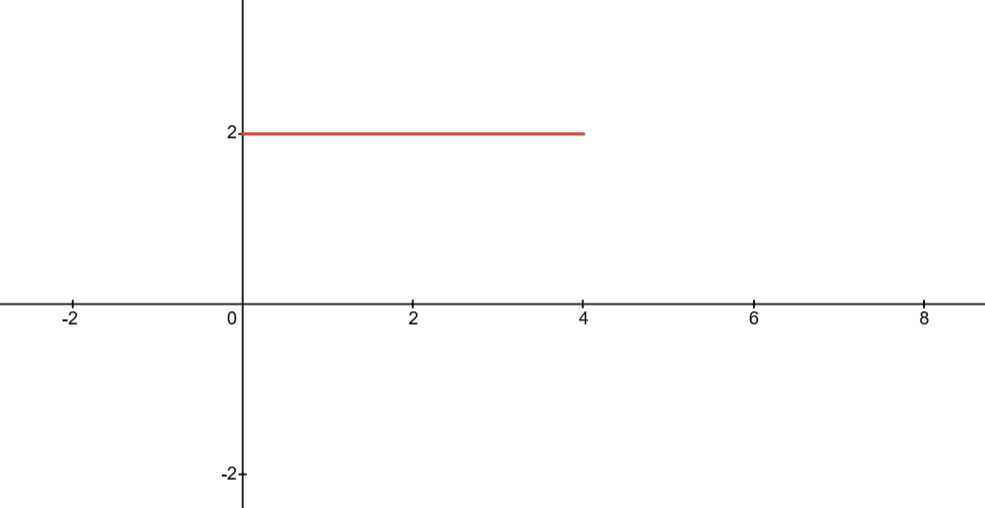
\includegraphics[width = 10cm]{change.png}
    \centering
    \caption{Graph of velocity-time}
\end{figure}

Solution:
To tackle this problem, recall the definition of velocity:
\[
v = \frac{d}{t}
\]
From the graph, we know that $v=2$ km/h and $t=4$ h, so distance is $d = vt = 8$km.

Coincidentally, it is also the area under the graph highlighted in red.

\begin{figure}[H]
    \centering
    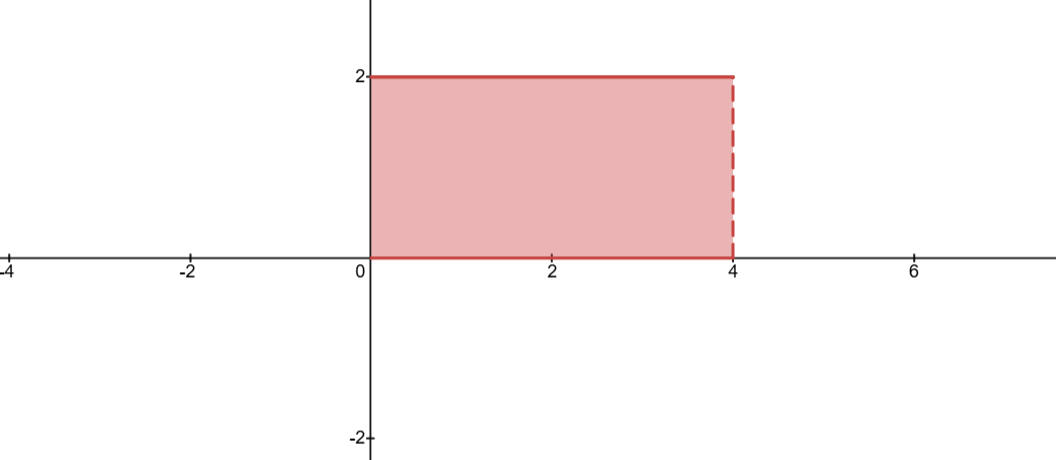
\includegraphics[width = 10cm]{highlightedChange.png}
\end{figure}


\end{document}